% !TEX root = ../IS.tex
\chapter{Introduction}
As the computing power of personal computers has increased, the depth and variety of interactive computer games has similarly increased. The earliest video games required two human players, and did not have any digital opponents. Games like Space Invaders and Pursuit introduced enemies which moved in set patterns; as time progressed, the intelligence of these enemies was improved with more intricate patterns (as in the space shooter Galaga) or in more heavily-scripted responses to inputs (as in the first-person shooter Half-Life) \cite{schw04}.

\begin{figure}[H]
  \centering
  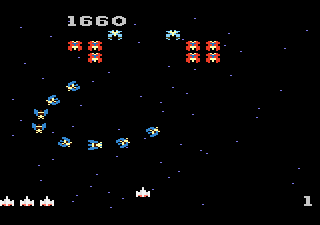
\includegraphics{figures/ExampleGalaga.png}
  \caption{A screenshot from the game \textit{Galaga}}
  \label{fig:Galaga}
\end{figure}
Galaga, for example, uses curves and loops in the flight paths of enemy spaceships, as can be seen in Figure \ref{fig:Galaga}. Compared to the straight lines of \textit{Space Invaders}, the spaceships became more challenging to hit. Furthermore, the spaceships were programmed to fire when the player was directly below them, while \textit {Space Invaders} had enemies shooting seemingly at random \cite{schw04}.\\

\lstset{caption={Section of AI script for Necron, a boss fight in the game \textit{Final Fantasy IX} \protect\cite{ff9necron}.}, language=ff9code, label={lst:ff9Necron}}
\begin{lstlisting}
set selectedattack = RandomAttack( attacklist )
if ( selectedattack == Flare )
    set SV_Target = RandomInTeam( NotMatching(SV_PlayerTeam[STATUS_CURRENT], PETRIFY | DEATH | ZOMBIE | REFLECT) & NotMatching(SV_PlayerTeam[STATUS_AUTO], REFLECT) )
elseif ( selectedattack == Holy )
    set SV_Target = RandomInTeam( NotMatching(SV_PlayerTeam[STATUS_CURRENT], PETRIFY | DEATH | ZOMBIE | REFLECT) & NotMatching(SV_PlayerTeam[STATUS_AUTO], REFLECT) )
elseif ( selectedattack == Meteor )
    set SV_Target = SV_PlayerTeam
\end{lstlisting}

In more recent titles, AI systems begin to show more intelligence. Some of this comes from more complex routines, as seen in the final boss of the game \textit{Final Fantasy IX}. The boss, named Necron, has a variety of possible actions, three of which are shown in Listing \ref{lst:ff9Necron}. A random attack is selected from the list in line 1. For two of these attacks, a random character in the player's team is selected, provided that they do not have one of the listed special statuses, in lines 3 and 5. Two of these statuses (PETRIFY and DEATH) refer to when a character controlled by the player can no longer perform actions of their own. The REFLECT status, on the other hand, prevents a player character from being affected by magic spells and inflicting the spell on its caster instead. These checks improve the percieved ``intelligence'' of the boss; the AI does not waste actions attacking incapacitated players or causing itself harm from reflected magic.\\

While the \textit{Final Fantasy IX} example employs predetermined choices (apart from some random selection), other forms of intelligence come from more open-ended coding. For example, stealth games feature guards who must react to a variety of situations. One technique for such AI is to use fuzzy logic \cite{schw04}.\\

In many role-playing games (RPGs), the heroes live in fantastical worlds and often have the ability to quickly heal themselves of their wounds with a quick potion or magic spell. While the player-controlled characters have these abilities, their AI-controlled opponents frequently do not. In rare cases where these enemies can heal themselves, this ability is often relegated to one-time uses determined by the game designers. This thesis concerns itself with designing an AI that can decide when it will use a healing ability, and use game theory to analyze the resulting game.